% Chapter Template

\chapter{Experimental set-up} % Main chapter title

\label{Chapter3} % Change X to a consecutive number; for referencing this chapter elsewhere, use \ref{ChapterX}

\lhead{Chapter 3. \emph{Experimental set-up}} % Change X to a consecutive number; this is for the header on each page - perhaps a shortened title

%--------------------------------------------------------
%	SECTION 1 - Motivation
%--------------------------------------------------------

\section{Motivation}

A large number of VAD algorithms proposed in the literature, the lack of standard methods for their evaluation and an abundance of speech and noise corpora makes it difficult to compare the results reported in the research papers. Therefore, the identification of an algorithm whose performance is objectively best is not possible without their proper benchmarking. In fact, it can be hypothesised that such objectively best algorithm does not exist since the performance of the algorithms will, at least to some extent, depend on the specific application and the encountered noise type. Another problem emerges from a variety of different hang-over schemes used in the experiments from the literature. These schemes can greatly affect the final VAD decisions and their use is especially important with the harmonicity based features which rely exclusively on the hang-over scheme for the detection of unvoiced phonemes. In order to unify the effect of hanging-over, the same scheme should be applied to all VAD features. Finally, some algorithms require estimation of the same values before the actual decision feature can be computed. For the algorithms chosen in this evaluation, these include noise power spectrum and pitch estimation. In order to reduce the performance bias coming from these estimates, the same procedures should be applied to all algorithms.

Therefore, the first aim of this chapter is to describe the implementation details of the selected VAD algorithms so that the differences in their operation can be easily identified\footnote{Ideally, they should differ only in the voicing features used for classification.}. Secondly, the speech and noise recordings as well as the corresponding procedure for obtaining the ground truth labels (for speech/non-speech) are presented so that the experiments can be repeated. For speech, a subset of the TIMIT \cite{TIMIT} database has been used. Recordings of various noise types have been taken from the NOISEX-92 \cite{NOISEX} database and added to the clean speech at various power levels.

%--------------------------------------------------------
%	SECTION 2 - VAD features
%--------------------------------------------------------

\section{VAD features}

Due to a large number of VAD features proposed in the literature, implementation and evaluation of all of them is impractical. However, a small number of features which appear to be noise-robust, based on different ideas and, ideally, recently published can be selected for comparison. In this evaluation, the features from the following VAD algorithms have been implemented:

\begin{itemize}
\item A Statistical Model-Based Voice Activity Detector \cite{Sohn} (hereinafter referred to as `Sohn')
\item Efficient Voice Activity Detection Algorithms Using Long-term Speech Information \cite{LTSD} (hereinafter referred to as `LTSD')
\item Entropy Based Voice Activity Detection in Very Noisy Conditions \citep{Renevey} (hereinafter referred to as `Entropy')
\item Noise Robust Voice Activity Detection Based on Periodic to Aperiodic Component Ratio \cite{PARADE} (hereinafter referred to as `PARADE')
\item Voice Activity Detection using Harmonic Frequency Components in Likelihood Ratio Test \cite{Tan} (hereinafter referred to as `Harmfreq')
\end{itemize}

In particular, the LTSD feature has been chosen because it is calculated taking into account multiple frames surrounding the one for which the decision is being made. Harmfreq is similar the Sohn feature, but calculates the likelihood ratio for the voiced phonemes only at the multiples of the fundamental frequency, hence it is a mixture of a LRT algorithm and a harmonicity based one. PARADE, on the other hand, is supposed to be robust to a variety of non-stationary noise types.

\subsection{Shared implementation parts}

The calculation of a number of VAD features requires prior estimation of some signal characteristics. In particular, Sohn, LTSD and Harmfreq need a noise power spectrum for the SNR estimate. Similarly, PARADE and Harmfreq require a pitch estimate in order to calculate the power of the signal at its multiples. In the original research papers either no procedure has been recommended (i.e. in Sohn \cite{Sohn} for noise PSD estimation) or different procedures have been suggested for estimation of the same property (i.e. pitch estimation in PARADE \cite{PARADE} and Harmfreq \cite{Tan}). In order to reduce the bias coming from potentially different estimation procedures, the same noise and pitch estimation algorithms have been applied to all VAD features. For the noise PSD, an implementation of the MMSE noise power estimator \cite{MMSEnoise} provided by VOICEBOX \cite{VOICEBOX} has been used. Similarly, the fundamental frequency in PARADE and Harmfreq has been estimated using PEFAC \cite{PEFAC}. Finally, before any processing, the incoming speech signal has been divided into 50 ms-long non-overlapping frames and windowed with a periodic Hanning window.

\subsection{Algorithm-specific implementation parts}

Apart from the same implementation parts used by different algorithms, there are parameters which are specific to some VAD features. Summary of the algorithm-specific implementation details is presented below:

\begin{itemize}
\item Sohn - the constant for decision-directed a priori SNR estimation is $\alpha = 0.95$
\item LTSD - the LTSE lookup into neighbouring frames is $N = 3$. Note that it is a smaller value than $N=6$ recommended in \cite{LTSD} due to a longer frame length and a lack of the overlap factor
\item PARADE - the number of harmonics is $\vartheta = 10$ or the maximum that fit in the resolution of the DFT
\item Harmfreq - $\alpha = 0.95$ (same as in Sohn). $\vartheta = 10$ or the maximum that fit in the resolution of the DFT (same as in PARADE). A frame is treated as voiced if the probability returned by PEFAC is greater than $0.5$
\end{itemize}

%--------------------------------------------------------
%	SECTION 3 - Hang-over scheme
%--------------------------------------------------------

\section{Hang-over scheme}
\label{sec:hang}

In order to reduce the differences in the final VAD decisions coming from different hang-over schemes, the same method has been applied to all evaluated VAD features, pseudo code of which is presented in Algorithm \ref{algo:hangover}. This is a modified and adapted to the chosen frame length version of the scheme originally published by ETSI in \cite{ETSIHangover}. This particular algorithm has been chosen because of its simplicity and good results achieved in the evaluation.

The main idea behind the scheme is to initialise the so-called \emph{hang-over timer} whenever the maximum number of consecutive speech decisions in the look-ahead buffer of $B$ frames is greater than $S_p$ (speech possible) or $S_l$ (speech likely). The proposed value for $B$ by ETSI is $7$ and the same has been used in this implementation. However, the values for parameters $S_p$, $S_l$, $L_s$ and $L_m$ were made smaller than the ones outlined in the standard, since the length of the processed signal frames is longer (i.e. 50 ms) and there is no overlap between them.

\begin{algorithm}
\textbf{INPUT:} $F$ - number of frames \\
\textbf{INPUT:} $V$ - VAD decisions prior to the hang-over scheme \\
\textbf{OUTPUT:} $hV$ - VAD decisions after the hang-over scheme
\begin{algorithmic}[1]
\STATE $B \leftarrow 7$ \COMMENT{buffer length}
\STATE $S_p \leftarrow 2$ \COMMENT{speech possible} 
\STATE $S_l \leftarrow 3$ \COMMENT{speech likely}
\STATE $L_s \leftarrow 5$ \COMMENT{short hang-over time}
\STATE $L_m \leftarrow 8$ \COMMENT{medium hang-over time}
\STATE
\STATE $T \leftarrow 0$ \COMMENT{hang-over timer}

\FOR{$i=1$ to $F-B+1$}
\STATE $CB \leftarrow V(i:i+B-1)$ \COMMENT{current buffer of VAD decisions}
\STATE $M \leftarrow$ maximum consecutive speech-present decisions in $CB$
\IF{$M \geqslant S_l$}
\STATE $T \leftarrow L_m$
\ELSIF{$M \geqslant S_p$ \AND $T < L_s$}
\STATE $T = L_s$
\ELSIF{$M < S_p$ \AND $T > 0$}
\STATE $T \leftarrow T-1$
\ENDIF
\IF{$T > 0$}
\STATE $hV(i) \leftarrow 1$
\ELSE
\STATE $hV(i) \leftarrow 0$
\ENDIF
\ENDFOR
\STATE $hV(F-B+2:F) \leftarrow V(F-B+2:F)$ \COMMENT{assign the pre hang-over decisions to the last B-1 frames}
\RETURN $hV$
\end{algorithmic}
\caption{Hang-over scheme used in all VAD algorithms}
\label{algo:hangover}
\end{algorithm}

%--------------------------------------------------------
%	SECTION 4 - Speech corpus
%--------------------------------------------------------

\section{Speech corpus}

There exists a number of speech corpora for evaluation of VAD and ASR. The choice of a specific corpus is a subjective matter and a large number of them have been used in the literature, making the results reported by the researchers not directly comparable. For the English language the TIMIT speech corpus \cite{TIMIT} seems to be the most widely used and hence has been selected as a source of utterances for this evaluation. There are a number of issues with the original recordings which need to be resolved so that the evaluation can be more accurate. These are:

\begin{itemize}
\item Single utterances are on average no longer than 4 seconds and hence too short for a proper VAD evaluation
\item The recordings contain a very small number of non-speech segments
\item There are differences in the average power between the utterances
\end{itemize}

In order to deal with the first two issues, a number of randomly chosen utterances from every dialect (i.e. DR1 to DR8) has been concatenated into a single speech recording, adding 2.5 seconds of silence at the beginning, ending and between the utterances. In an attempt to equalise the power, the amplitude of each utterance has been normalised such that the average power per sample of all of them is equal. This is important because if the concatenated utterances differed in the average power level, after adding the noise, the one with initially higher power could be easily detected by almost any VAD procedure while the detection of the other one would be very difficult due to the much lower segmental/short-time SNR.

For a proper VAD evaluation, the ground truth speech/non-speech labels need to be obtained. While this might seem like a simple task, it actually includes a degree of subjectivity. Consider Figure \ref{fig:groundtruth} where the speaker first makes a short pause between words and then, after the utterance, takes a breath while still standing near the microphone. Whether the first segment should be classified as speech, since it clearly forms a part of a longer utterance, or silence, since if considered in isolation, it does not exhibit any obvious speech characteristics, is a matter of choice. In this work, all such segments and alike have been treated as integral parts of the utterances and hence classified as speech in the ground truth labels. Obviously, the breath part is not speech and should be treated as such. The initial labels have been obtained by a simple energy VAD and examined visually, making necessary manual changes to any obviously misclassified segments, taking into account the decisions described before.

\begin{figure}[htbp]
	\centering
		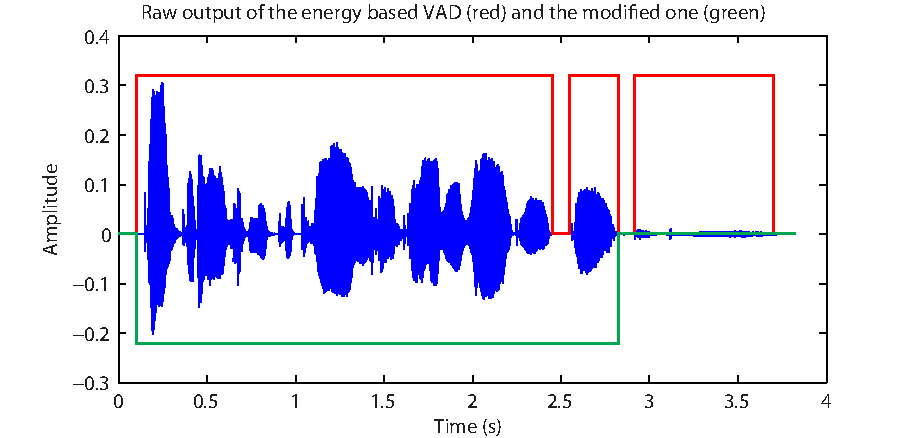
\includegraphics[width=1.0\columnwidth]{Figures/Chapter3/groundtruthbold.pdf}
		\rule{37em}{0.5pt}
	\caption[Raw and modified outputs from the energy based VAD used as ground truth labels]{Raw and modified outputs from the energy based VAD used as ground truth labels}
	\label{fig:groundtruth}
\end{figure}

%--------------------------------------------------------
%	SECTION 5 - Noise corpus and SNR
%--------------------------------------------------------

\section{Noise corpus and SNR}

Similarly to the speech corpora, there exists a large number of noise databases which are commonly used for evaluation of speech processing algorithms. In this evaluation, most noise types have been taken from the NOISEX-92 \cite{NOISEX} corpus with the exception of the babble noise which has been adapted from the Nato Noise \cite{Nato} package. Also, the white noise has been generated\footnote{The white noise has been generated only once. The exact same samples have been used for evaluation of all algorithms.} by MATLAB's \texttt{randn} function which returns samples of the naturally distributed Gaussian random variable with zero mean\footnote{In this case, the variance, which by default is 1, is irrelevant since the noise is scaled before addition to the clean speech signal anyway.}. The complete list of the noise types used in this evaluation is: white, car, spchspect, babble, opsroom and factory.

In order to evaluate the algorithms' performance under different conditions, the clean speech and noise signals need to be scaled to the desired SNR. This is achieved by the following procedure which ensures the correct power of noise relative to the speech:

\begin{enumerate}
\item Calculate the active level of the clean speech signal\footnote{The active level of a speech signal is defined to be its average power during intervals when speech is present.} $P_s$
\item Calculate the average power of noise $P_n$
\item Calculate the scaling constant for noise as $\sqrt{\frac{P_s}{10^{\text{SNR}/10} \times P_n}}$
\item Multiply each noise sample by the scaling constant
\item Add the scaled noise signal to the clean speech signal
\end{enumerate}

%--------------------------------------------------------
%	SECTION 6 - Summary
%--------------------------------------------------------

\section{Summary}

This chapter described the important considerations and choices which have been made with respect to the experimental set-up. An effort has been made to unify as many of the algorithm's parts as possible so that the actual voice detection features can be compared objectively. All algorithms will be evaluated on the same speech and noise recordings under various SNRs. Finally, the same hang-over scheme will be applied to all features in order to remove the variance in the results coming from the performance of different schemes as opposed to the quality of the voice detection features.